\chapter{Środowisko symulacyjne}
\label{cha:rozdzial4}

Gdy projektowano pierwsze maszyny, które miały wykonywać konkretne zadania, opierano
się na dokładnych modelach matematycznych opisujących fizykę. Nie istniały narzędzia
do weryfikacji skuteczności działania danego urządzenia. Dopiero rozwój technologii
komputerowych i wzrost mocy obliczeniowej procesorów umożliwił bardzo szybką 
weryfikację stworzonych maszyn na komputerach, które w kilka sekund były w stanie 
sprawdzić poprawność obliczeń. Duże znaczenie symulacje zaczęły odgrywać kiedy
testowanie projektowanych maszyn mogło sprawiać zagrożenia dla ludzi czy samego
środowiska, w którym były testowane.

Ze względu na coraz niższą cenę sprzętu komputerowego i rozwojowi oprogramowania,
coraz więcej osób może w swoich domach uruchamiać modele wielu urządzeń bez ryzyka
uszkodzenia czegokolwiek i móc prowadzić swoje badania. W poniższej pracy konieczne
było zastosowanie takiego środowiska symulacyjnego, ponieważ testowane rozwiązania
są nowe i agenci uczenia motywowanego mogą czasem wykonywać czynności, które nie
były uwzględnione przez projektanta, zgodnie z tabelą \ref{tab:ml_vs_rl}.

W poniżej pracy uczenie motywowane będzie testowane na robocie mobilnym w środowisku
symulacyjnym Gazebo Sim \cite{gazebo_sim_website}.

\section{Symulator Gazebo}

Rozwój symulatora Gazebo rozpoczął się jesienią 2002 roku na Uniwersytecie 
Południowej Kalifornii. Oryginalnymi twórcami byli dr Andrew Howard i jego 
uczeń Nate Koenig. Koncepcja symulatora o wysokiej wierności wynikała z potrzeby 
symulacji robotów w środowiskach zewnętrznych w różnych warunkach. 
Jako komplementarny symulator do Stage, nazwa Gazebo została wybrana jako 
struktura najbliższa scenie zewnętrznej. Nazwa utknęła pomimo faktu, że 
większość użytkowników Gazebo symuluje środowisko wewnętrzne.

\begin{figure}[h]
    \centering
    \includegraphics[width=0.3\linewidth]{rozdzial5/images/gazebo_logo}
    \caption{Logo Gazebo Sim. Źródło: \cite{gazebo_sim_website}.}
    \label{fig:gazebo_logo}
\end{figure}

Symulator ten ma zintegrowane silnik fizyki ODE (Open Dynamics Engine). Wykorzystuje
renderowanie korzystając z OpenGL. Dzięki temu możeliwe jest symulowanie wielu 
rodzajów sensorów:

\begin{itemize}
    \item ciśnieniomierz,
    \item wysokościomierz,
    \item kamera (RGB, głębi),
    \item czujnik kontaktu (dotyku),
    \item czujnik nacisku,
    \item GPS,
    \item lidar,
    \item skaner laserowy,
    \item IMU (ang. \textit{inertial measurement unit}),
    \item magnetometr,
    \item czujnik odległości,
    \item inne.
\end{itemize}

Tak duży zasób czujników umożliwia sprawdzanie na wiele sposobów jaki zestaw 
sensorów może być wykorzystany dla konkretnych celów oraz sprawia, że testowanie
nowych funkcjonalności bez ryzyka uszkodzenia robota czy środowiska. 

Graficzny interfejs umożliwia szybkie projektowanie nowych robotów czy elementów
środowiska. Wygląd głównego okna, w którym wykonywana jest większość pracy
podczas projektowania środowiska symulacyjnego pokazano na rysunku 
\ref{fig:gazebo_main_window}.

\begin{figure}[h]
    \centering
    \includegraphics[width=0.7\linewidth]{rozdzial5/images/gazebo_main_window}
    \caption{Główne okna symulatora Gazebo. Źródło: opracowanie własne.}
    \label{fig:gazebo_main_window}
\end{figure}

Dodatkowowo w Gazebo oprócz silnika fizycznego ODE można skorzystać także z innych
bardzo popularnych silników fizyczny jak: Bullet. Dzięki rzeczywistemu renderowaniu
sceny w kamerach możliwe jest testowanie systemów wizyjnych. Takie na pewno
muszą być zastosowane dla agenta z uczeniem motywowanym, ponieważ to jeden
z podstawowych sensorów stosowanych przez człowieka na etapie poznawania nowego
środowiska.

Środowisko Gazebo Sim składa się z kilku elementów, które sprawiają, że możliwe
jest uruchomienie symulacji robota. Są to zgodnie z \cite{gazebo_components}.

\begin{itemize}
    \item \textbf{World files} -- pliki zawierające opis danego środowiska, 
    w którym robot ma działać, można w nich modyfikować parametry świata, 
    np. siłę grawitacji,
    \item \textbf{Model files} -- pliki w formacie SDF zawierające opisy 
    struktury robota,
    \item \textbf{Environment variables} -- zmienne środowiskowego, które 
    umożliwiają w prosty sposób uruchamiać Gazebo i ładować modele robotów 
    do symulacji,
    \item \textbf{Gazebo Server} -- główny program symulacji, który wykonuje 
    wszelkie obliczenia tj. liczenie kolizji, symulowanie czujników,
    \item \textbf{Graphical Client} -- umożliwia wyświetlanie wyników 
    obliczeń z serwera Gazebo,
    \item \textbf{Plugins} -- małe biblioteki, które umożliwiają w prosty 
    sposób wchodzić w interakcję w symulacją poprzez tworzenie własnych 
    sensorów czy wtyczek modyfikujących parametry świata z poziomu kodu.
\end{itemize}

Architektura całego systemu umożliwia proste projektowanie sensorów, robotów
czy całych środowisk do symulowania różnych scenariuszy środowiska jak 
parametry, np. siła grawitacji czy opory powietrza, jeżeli symulowane są roboty
latające jak drony. 

Gazebo używa rozproszonej architektury z rozdzielonymi bibliotekami do 
symulacji fizyki, renderowania sceny, interfejsu użytkownika, komunikacji i 
generowaniu sensorów. Dodatkowo w celu uruchomienia wszystkich możliwości 
symulatora, wcześniej wspomnianych: \textit{gzserver} do symulowania fizyki, 
renderowania i sensorów oraz \textit{gzclient}, który umożliwia wyświetlanie 
interfejsu użytkownika. Elementy architektury Gazebo przedstawiono na rysunku 
\ref{fig:gazebosystemarchitecture}:

\begin{figure}
	\centering
	\includegraphics[width=0.7\linewidth]{rozdzial5/images/gazebo_system_architecture}
	\caption{Architektura systemu Gazebo. Źródło: opracowanie własne.}
	\label{fig:gazebosystemarchitecture}
\end{figure}


\section{Wizualizacja w RViz}
Kolejnym bardzo przydatnym narzędziem stosowanym przy rozwijaniu oprogramowania na roboty
jest program RViz. Służy on do wizualizacji danych z różnych sensorów w czytelny
i przejrzysty sposób. Dostarcza także szereg tzw. interaktywnych markerów, z którymi
użytkownik może wchodzić w interakcję i wydawać komendy do robota, który działa na
innej maszynie. 

Podgląd danych z kamer czy chmur punktów oraz połączenie przez sieć z robotem, możliwe
jest zdalne sterowanie robotem przy jednoczesny wglądzie do aktualnych danych z kamer
czy odometrii robota. RViz to bardzo prosty przykład interfejsu człowiek komputer
HMI (ang. \textit{human -- machine interface}) znany szeroko ze sterowników przemysłowych.
Sam program dostarcza API (ang. \textit{application programming interface}), który umożliwia
rozszerzanie dostępnych funkcjonalności o bardziej dostosowane do wymagań danego projektu.

\begin{figure}[H]
	\centering
	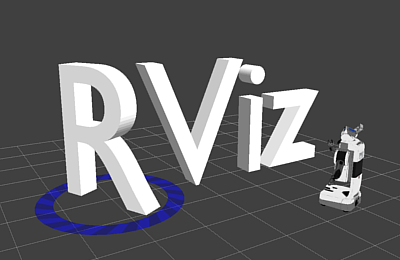
\includegraphics[width=0.7\linewidth]{rozdzial5/images/rviz_logo}
	\caption{Logo programu RViz oraz robot PR2. Żródło: {\cite{rviz}}}
	\label{fig:rvizlogo}
\end{figure}

W tym projekcie został on zastosowany do podglądu aktualnej pozycji robota na przygotowanej
mapie oraz wizualizacji samej mapy, co obrazuje figura \ref{fig:rvizsample}. 

\begin{figure}[H]
	\centering
	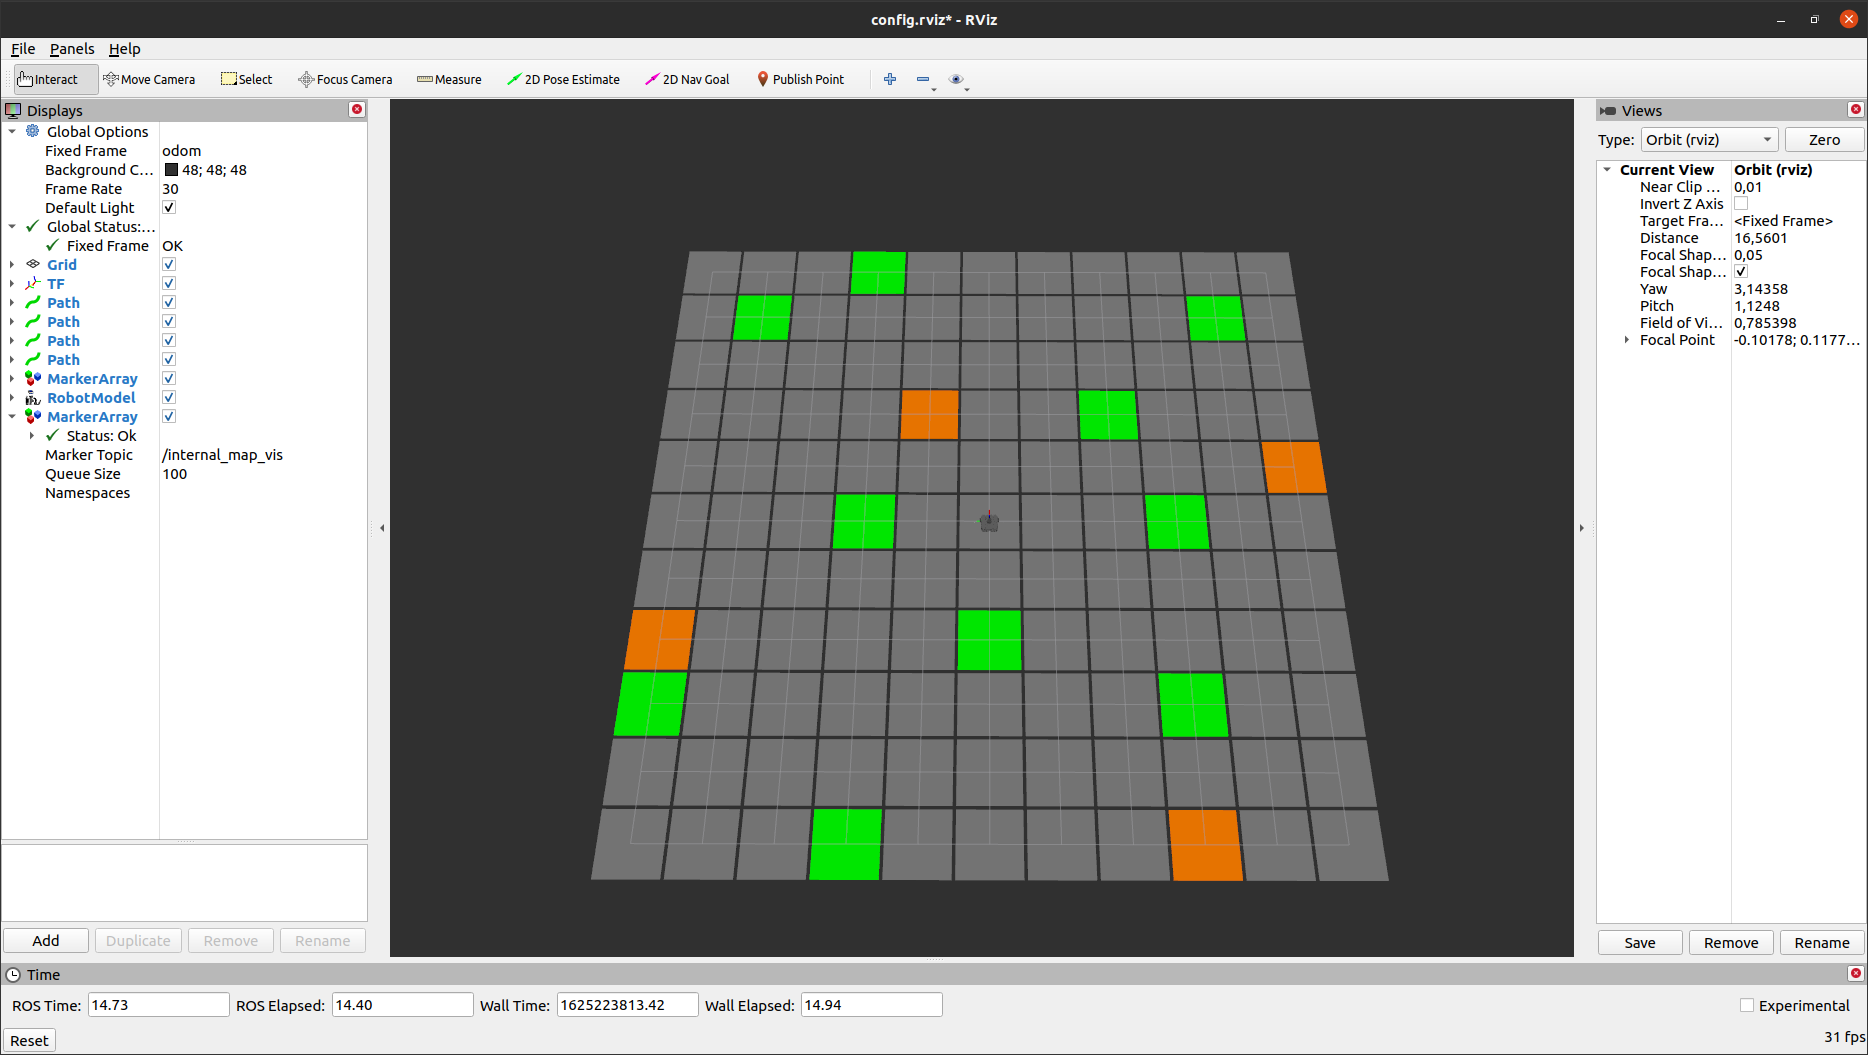
\includegraphics[width=0.9\linewidth]{rozdzial5/images/rviz_sample}
	\caption{Przykładowy zrzut ekranu aplikacji RViz z wyświetlonym modelem robota i mapą.
	Źródło: opracowanie własne.}
	\label{fig:rvizsample}
\end{figure}

\section{Zbiór bibliotek RQT}
Ostatnim narzędziem, które znacznie usprawnia pracę w trakcie rozwijania oprogramowania
na wszelkiego rodzaju roboty jest platforma programistyczna (ang. \textit{framework}) RQT.
Oparta ona została na szeroko znanej bibliotece QT, służącej do projektowania interfejsów
graficzny tzw. GUI (ang. \textit{graphical user interface}). Stosując RQT można łatwo
projektować interfejsy graficzne do wygodnego sterowania robotem. Dzięki temu, że RQT
korzysta z QT, możliwe jest stosowanie narzędzi dostarczanych przez QT, tj. QT Designer.
Platforma RQT dostarcza podstawowe interfejsy, dzięki którym nasza aplikacja ma bezpośrednie
połączenie do systemu robotycznego ROS, który został użyty w tym projekcie. Każda z takich
aplikacji zachowuje się jak plugin do RQT. Możemy otworzyć wiele różnych pluginów
w jednym oknie, aranżować ich rozmieszczenie w oknie aplikacji oraz dynamiczne
włączać i wyłączać. Przykładowy widok okna RQT na obrazku \ref{fig:rqtsample} (proszę
zwrócić uwagę na plugin z załadowaną stroną internetową w lewym górnym rogu).

\begin{figure}[H]
	\centering
	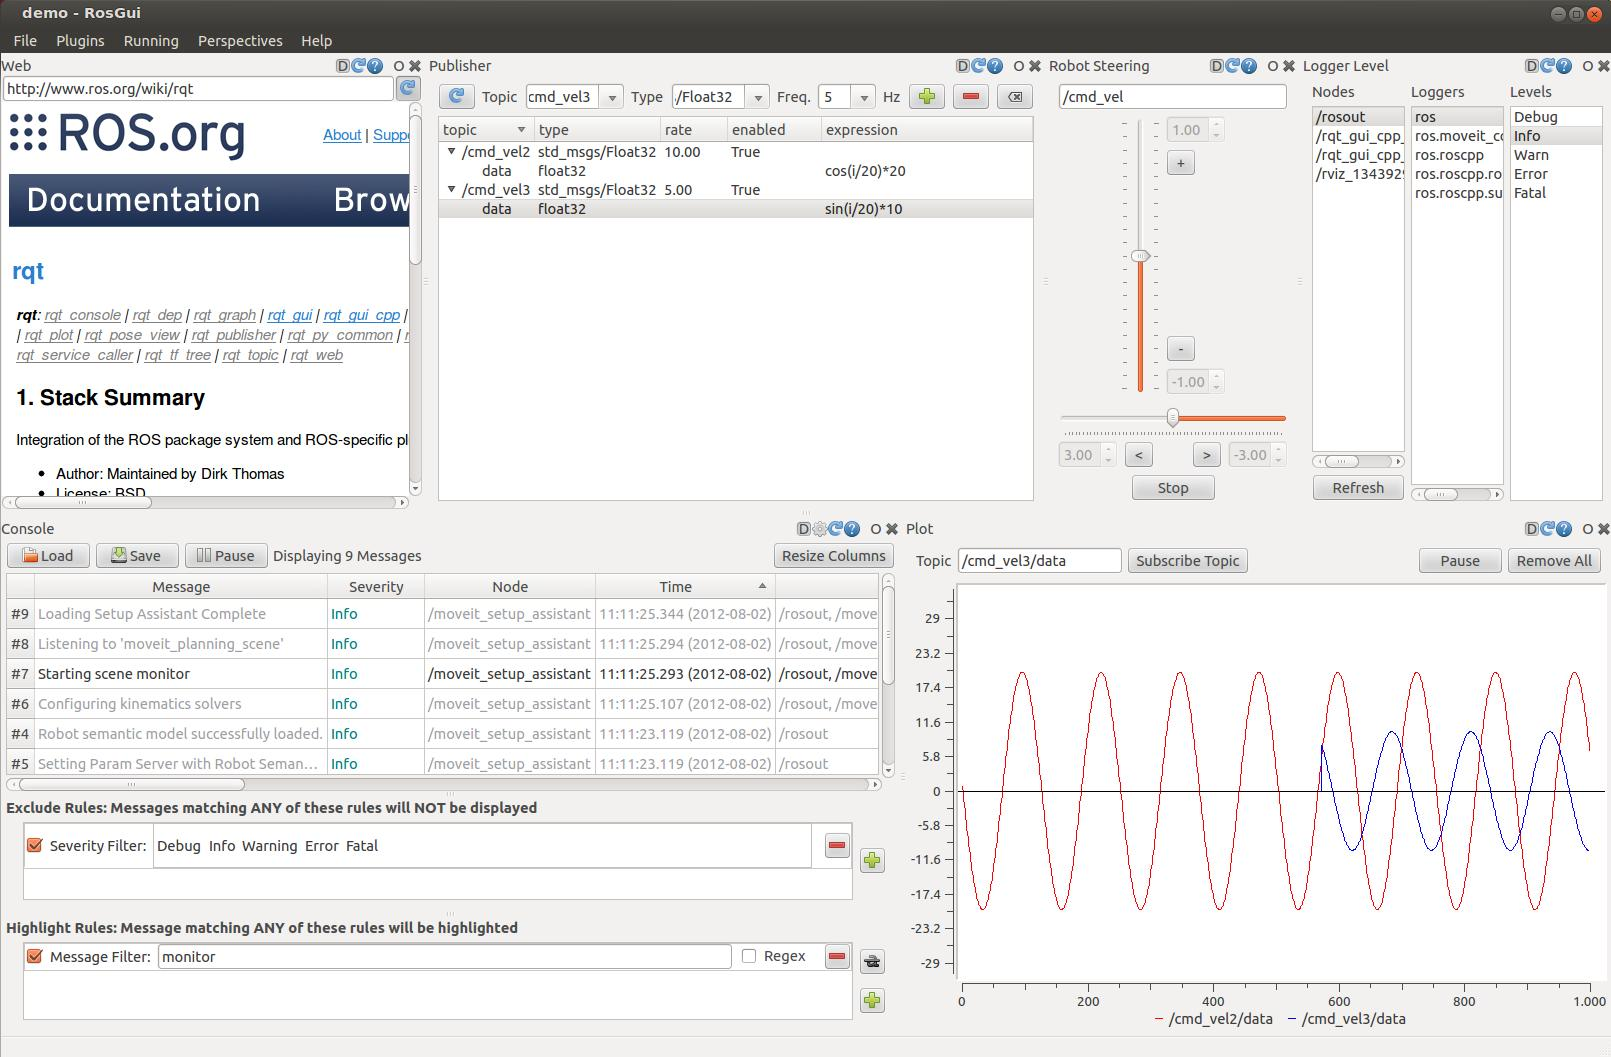
\includegraphics[width=0.8\linewidth]{rozdzial5/images/rqt_sample}
	\caption{Przykładowy widok załadowanych pluginów do RQT. Źródło: \cite{rqt}}
	\label{fig:rqtsample}
\end{figure}

